\documentclass[a4]{article}
\pagestyle{myheadings}

%%%%%%%%%%%%%%%%%%%
% Packages/Macros %
%%%%%%%%%%%%%%%%%%%
\usepackage{mathrsfs}


\usepackage{fancyhdr}
\pagestyle{fancy}
\lhead{}
\chead{}
\rhead{}
\lfoot{}
\cfoot{} 
\rfoot{\normalsize\thepage}
\renewcommand{\headrulewidth}{0pt}
\renewcommand{\footrulewidth}{0pt}
\newcommand{\RomanNumeralCaps}[1]
{\MakeUppercase{\romannumeral #1}}

\usepackage{amssymb,latexsym}  % Standard packages
\usepackage[utf8]{inputenc}
\usepackage[russian]{babel}
\usepackage{MnSymbol}
\usepackage{amsmath,amsthm}
\usepackage{indentfirst}
\usepackage{graphicx}%,vmargin}
\usepackage{graphicx}
\graphicspath{{pictures/}} 
\usepackage{verbatim}
\usepackage{color}









\DeclareGraphicsExtensions{.pdf,.png,.jpg}% -- настройка картинок

\usepackage{epigraph} %%% to make inspirational quotes.
\usepackage[all]{xy} %for XyPic'a
\usepackage{color} 
\usepackage{amscd} %для коммутативных диграмм


\newtheorem{Lemma}{Лемма}[section]
\newtheorem{Proposition}{Предложение}[section]
\newtheorem{Theorem}{Теорема}[section]
\newtheorem{Corollary}{Следствие}[section]
\newtheorem{Remark}{Замечание}[section]
\newtheorem{Definition}{Определение}[section]
\newtheorem{Designations}{Обозначение}[section]




%%%%%%%%%%%%%%%%%%%%%%%% 
%Сношение с оглавлением% 
%%%%%%%%%%%%%%%%%%%%%%%% 
\usepackage{tocloft} 
\renewcommand{\cftdotsep}{2} %частота точек
\renewcommand\cftsecleader{\cftdotfill{\cftdotsep}}
\renewcommand{\cfttoctitlefont}{\hspace{0.38\textwidth} \LARGE\bfseries} 
\renewcommand{\cftsecaftersnum}{.}
\renewcommand{\cftsubsecaftersnum}{.}
\renewcommand{\cftbeforetoctitleskip}{-1em} 
\renewcommand{\cftaftertoctitle}{\mbox{}\hfill \\ \mbox{}\hfill{\footnotesize Стр.}\vspace{-0.5em}} 
\renewcommand{\cftsubsecfont}{\hspace{1pt}} 
\renewcommand{\cftparskip}{3mm} %определяет величину отступа в оглавлении
\setcounter{tocdepth}{5} 




\addtolength{\textwidth}{0.7in}
\textheight=630pt
\addtolength{\evensidemargin}{-0.4in}
\addtolength{\oddsidemargin}{-0.4in}
\addtolength{\topmargin}{-0.4in}

\newcommand{\empline}{\mbox{}\newline} 
\newcommand{\likechapterheading}[1]{ 
	\begin{center} 
		\textbf{\MakeUppercase{#1}} 
	\end{center} 
	\empline} 

\makeatletter 
\renewcommand{\@dotsep}{2} 
\newcommand{\l@likechapter}[2]{{\bfseries\@dottedtocline{0}{0pt}{0pt}{#1}{#2}}} 
\makeatother 
\newcommand{\likechapter}[1]{ 
	\likechapterheading{#1} 
	\addcontentsline{toc}{likechapter}{\MakeUppercase{#1}}} 





\usepackage{xcolor}
\usepackage{hyperref}
\definecolor{linkcolor}{HTML}{000000} % цвет ссылок
\definecolor{urlcolor}{HTML}{AA1622} % цвет гиперссылок

\hypersetup{pdfstartview=FitH,  linkcolor=linkcolor,urlcolor=urlcolor, colorlinks=true}



\def \newstr {\medskip \par \noindent} 



\begin{document}
	\def\contentsname{\LARGE{Содержание}}
	\thispagestyle{empty}
	\begin{center} 
		\vspace{2cm} 
		{\Large \sc Санкт-Петербургский Политехнический Университет}\\
		\vspace{2mm}
		{\Large\sc Петра Великого}\\
		\vspace{1cm}
		{\large \sc Институт прикладной математики и механики\\ 
			\vspace{0.5mm}
			\textsc{}}\\ 
		\vspace{0.5mm}
		{\large\sc Кафедра $"$Прикладная математика$"$}\\
		\vspace{15mm}
		
		
		{\sc \textbf{Отчёт\\
			Лабораторная работа №$1$\\
			по дисциплине\\
			"Математическая статистика"}
			\vspace{6mm}
			
		}
		\vspace*{2mm}
		
		
		\begin{flushleft}
			\vspace{4cm}
			\sc Выполнил студент:\\
			\sc Салихов С.Р.\\
			\sc группа: 3630102/70401\\
			\vspace{1cm}
			\sc Проверил:\\
			\sc к.ф-м.н., доцент\\
			\sc Баженов Александр Николавич
			\vspace{20mm}
		\end{flushleft}
	\end{center} 
	\begin{center}
		\vfill {\large\textsc{Санкт-Петербург}}\\ 
		2020 г.
	\end{center}
	
	\newpage
	\pagestyle{plain}
	
	%\begin{center}
	%\begin{abstract} 
	
	%\end{abstract}
	
	%\end{center}
	
	\newpage
	\tableofcontents{}
	\newpage
	\listoffigures
	\newpage
	
	
	\section{Постановка задачи}
	
	Для 5-ти рапределений:\\
		Нормальное распределение $N(x,0,1)$\\
		Распределение Коши $C(x,0,1)$\\
		Распределение Лапласа $L( x,0,\frac{1}{\sqrt{2}})$\\
		Распределение Пуассона $P(k, 10)$\\
		Равномерное Распределение $U(x,-\sqrt{3}, \sqrt{3})$\\
		
		Сгенерировать выборки размером 10, 50 и 1000 элементов.
		Построить на одном рисунке гистограмму и график плотности распределения.
		
	
	\section{Теория}
		\subsection{Распределения}
		
			\begin{equation}\label{eqn:normal}
			N(x,0,1) = \frac{1}{\sqrt{2\pi}}e^{-\frac{x^2}{2}}
			\end{equation} 
			
			\begin{equation}\label{eqn:cauchy}
			C(x,0,1) = \frac{1}{\pi(1+x^2)}
			\end{equation}
			
			\begin{equation}\label{eqn:laplace}
			L\left( x,0,\frac{1}{\sqrt{2}}\right) = \frac{1}{\sqrt{2}}e^{-\sqrt{2}\vert x\vert}
			\end{equation}
			
			\begin{equation}\label{eqn:poisson}
			P(k,10) = \frac{10^k}{k!}e^{-10}
			\end{equation}  
			
			\begin{equation}\label{eqn:uniform}
			U(x,-\sqrt{3}, \sqrt{3}) = 
			\begin{cases}
			\frac{1}{2\sqrt{3}} &\vert x\vert \leqslant \sqrt{3}\\
			0 &\vert x\vert > \sqrt{3}
			\end{cases}
			\end{equation}
		
		\subsection{Гистограмма}
			\subsubsection{Определение}
				Гистограмма в математической статистике — это функция, приближающая
				плотность вероятности некоторого распределения, построенная на основе
				выборки из него.

		
			\subsubsection{Графическое описание}
				Графически гистограмма строится следующим образом. Сначала множество значений, которое может принимать элемент выборки, разбивается на
				несколько интервалов. Чаще всего эти интервалы берут одинаковыми, но
				это не является строгим требованием. Эти интервалы откладываются на
				горизонтальной оси, затем над каждым рисуется прямоугольник. Если все
				интервалы были одинаковыми, то высота каждого прямоугольника пропорциональна числу элементов выборки, попадающих в соответствующий
				интервал. Если интервалы разные, то высота прямоугольника выбирается
				таким образом, чтобы его площадь была пропорциональна числу элементов
				выборки, которые попали в этот интервал.
			\subsubsection{Использование}
				Гистограммы применяются в основном для визуализации данных на начальном этапе статистической обработки.
				Построение гистограмм используется для получения эмпирической оценки
				плотности распределения случайной величины. Для построения гистограммы наблюдаемый диапазон изменения случайной величины разбивается на
				несколько интервалов и подсчитывается доля от всех измерений, попавшая
				в каждый из интервалов. Величина каждой доли, отнесенная к величине
				интервала, принимается в качестве оценки значения плотности распределения на соответствующем интервале.
				
	\section{Реализация}
	Для генерации выборки был использован $Python\;3.7$: модуль $random$ библиотеки $numpy$ для генерации случайных чисел с различными распределениями и библиотека $matplotlib$ для построения графиков и гистограмм.
	\section{Результаты}
		\subsection{Гистограмма и график плотности распределения}	
			\begin{center}
				
				\begin{figure}[h]
					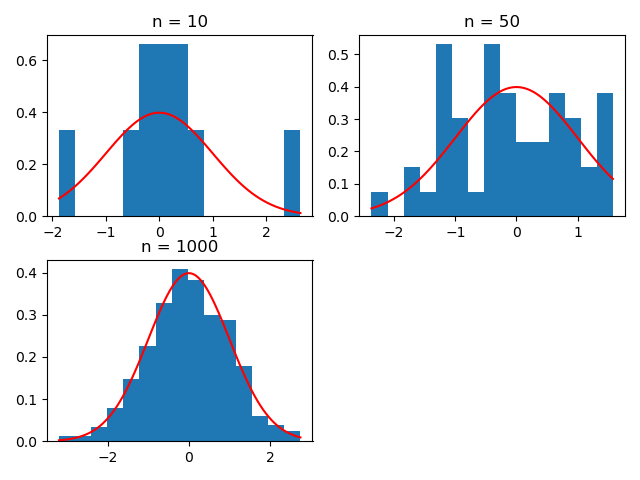
\includegraphics[width=\textwidth]{normal.png} 
					\caption[Нормальное распределение]{Нормальное распределение}
				\end{figure}
				
				\begin{figure}
					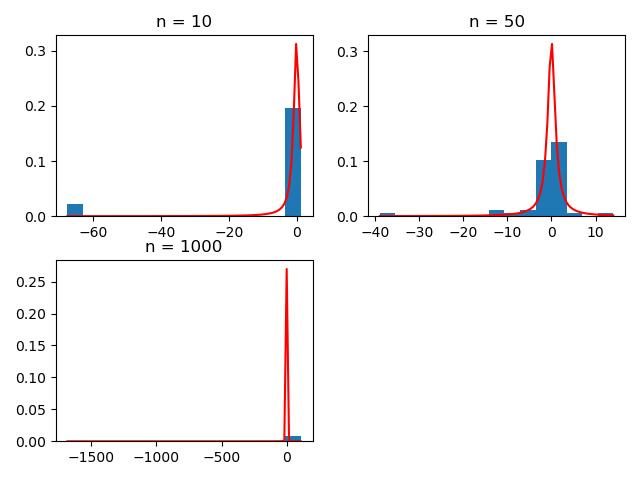
\includegraphics[width=\textwidth]{cauchy.png}
					\caption[Распределение Коши]{Распределение Коши}
				\end{figure}
		
				\begin{figure}
					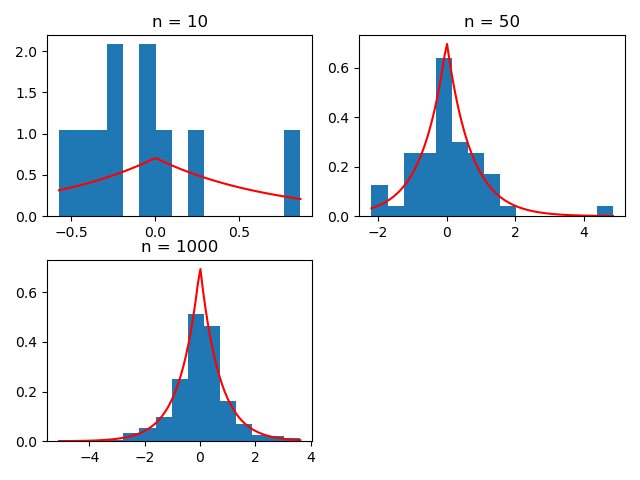
\includegraphics[width=\textwidth]{laplace.png}
					\caption[Распределение Лапласа]{Распределение Лапласа}
				\end{figure}
			
				\begin{figure}
					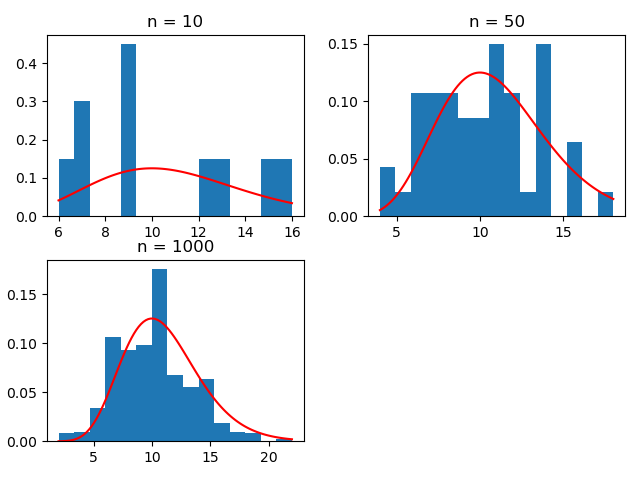
\includegraphics[width=\textwidth]{poisson.png}
					\caption[Распределение Пуассона]{Распределение Пуассона}
				\end{figure}
				\begin{figure}
					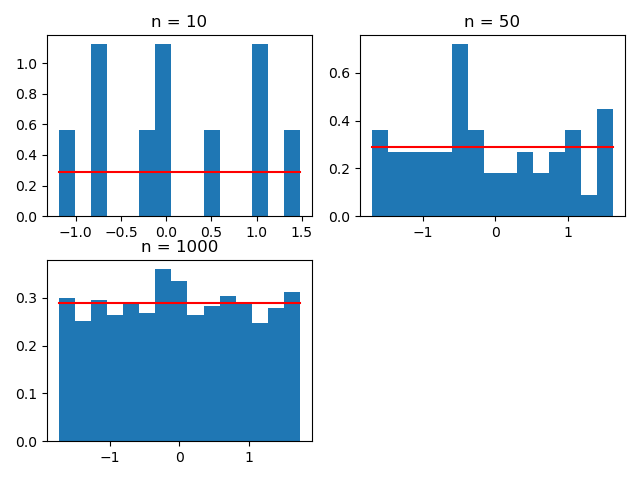
\includegraphics[width=\textwidth]{uniform.png}
					\caption[Равномерное распределение]{Равномерное распределение}
				\end{figure}
	
		\end{center}
		
			\subsection{Характристики положения и рассеяния}
		
	\section{Обсуждение}
		\subsection{Гистограмма и график распределения}
		Благодаря полученным графикам можно увидеть, что: чем больше выборка, тем график плотности более близок к гистограмме. При малой выборке, наблюдается скачок значений в гистограмме.
	
	\section{Литература}
	
	\href{https://physics.susu.ru/vorontsov/language/numpy.html}{Модуль numpy}
	
	\section{Приложения}
	
	\href{https://github.com/LuciusGen/Matstat/blob/master/Lab1/Lab1.py}{Код лаборатрной}
	
	\href{https://github.com/LuciusGen/Matstat/blob/master/Lab1/document.tex}{Код отчёта}
	
\end{document}